\documentclass[11pt,a4paper]{article}

\usepackage[margin=1in]{geometry}
\usepackage{amsmath,amssymb,amsthm,mathtools}
\usepackage{booktabs,array,tabularx}
\usepackage{graphicx}
\usepackage{enumitem}
\usepackage{hyperref}
\usepackage{xcolor}
\usepackage{microtype}
\usepackage{caption}
\usepackage{subcaption}
\usepackage{cite}
\usepackage{float}
\usepackage{placeins}

\hypersetup{
  colorlinks=true,
  linkcolor=blue!65!black,
  citecolor=blue!65!black,
  urlcolor=blue!65!black
}

\newtheorem{theorem}{Theorem}
\newtheorem{proposition}{Proposition}
\newtheorem{lemma}{Lemma}
\newtheorem{remark}{Remark}
\newtheorem{definition}{Definition}

\newcommand{\R}{\mathbb{R}}
\newcommand{\E}{\mathbb{E}}
\newcommand{\Lap}{\operatorname{Laplace}}
\newcommand{\MSE}{\operatorname{MSE}}
\newcommand{\Var}{\operatorname{Var}}
\newcommand{\argmin}{\operatorname*{arg\,min}}

\title{\textbf{Fair Mean Estimation under Heterogeneous Privacy Costs:\\Mechanism Design, Optimization, and Empirical Dynamics}\\[0.5em]
\large Research Report for Machine Learning and Incentives}
\author{\textbf{Research Study Notes}}
\date{November 2026}

\begin{document}
\maketitle

\begin{abstract}
We study the problem of acquiring private data from strategic individuals belonging to heterogeneous demographic groups to estimate a population mean under differential privacy (DP). We build on the optimal central mechanism-design framework of Fallah et al.~\cite{fallah2023optimal} and extend it to incorporate demographic fairness. We examine how a platform-level group-conditional Mean Squared Error (MSE) disparity penalty alters optimal privacy allocations, payment structures, and accuracy trade-offs. Using a scalable numerical optimization pipeline that solves the joint weight-budget minimization problem, we conduct comprehensive experiments spanning homogeneous privacy costs, inter-group cost disparities, and heavy-tailed versus bounded cost distributions (Uniform, Log-Normal, and Truncated Normal). Notably, we empirically validate and analytically characterize the \emph{cheaper fairness phenomenon} a curious case where introducing a fairness penalty \emph{reduces} total platform procurement expenditures while reducing group error disparity.
\end{abstract}

\newpage

%=============================================================================
\section{Introduction and Problem Motivation}
%=============================================================================

In modern machine learning and data economics, platforms routinely acquire sensitive data from individuals who experience heterogeneous privacy costs. The results of the aggregation of this data benefit the individuals as well. Differential privacy (DP) guaranties that individuals' private attributes are safeguarded~\cite{dwork2006calibrating,dwork2014algorithmic}. The current baseline in central differentially private data acquisition balances statistical accuracy (minimizing Mean Squared Error, $\MSE$) against total monetary compensation paid to participants according to their cost to privacy ~\cite{fallah2023optimal}. However, in populations comprising of distinct demographic groups (e.g., socioeconomic, geographic, or ethnic cohorts), standard accuracy-maximizing DP estimators may suffer from severe \textbf{disparities} as follows:

\begin{enumerate}
    \item \textbf{Sample Size Disparities:} Majority groups dominate the objective function, causing the estimator to prioritize majority accuracy at the expense of higher group-conditional error for underrepresented minorities.
    \item \textbf{Privacy Cost Disparities:} When one demographic group faces systematically higher privacy concerns (e.g., stigmatized conditions, marginalized populations), standard cost-minimizing procurement starves that group of privacy budget, forcing them into higher privacy loss or severely under-weighting their observations.
\end{enumerate}

To rectify this, we investigate a Fairness Extension of Heterogeneous Privacy Allocation described in \cite{fallah2023optimal} where the platform objective gets an additional penalty proportional to the squared difference between MSEs in each group. The primary objectives of this report are:
\begin{itemize}[leftmargin=1.5em]
    \item Concisely formalize the two-group statistical and mechanism-design setting with heterogeneous privacy costs.
    \item Give implementation details of a constrained optimization engine solving the joint allocation $(w^*, S^*)$.
    \item Systematically execute and analyze five key experimental regimes covering homogeneous and heterogeneous costs, varying demographic proportions, and different cost distribution geometries.
    \item Unpack the analytical intuition behind the curious \emph{cheaper fairness} effect, where requiring group fairness saves the platform money.
\end{itemize} 

%=============================================================================
\section{Theoretical Framework}
%=============================================================================

\subsection{Estimator and Privacy Allocation}

We consider a population of $n$ participants partitioned into two non-empty demographic groups $\mathcal{A}$ and $\mathcal{B}$, with sizes $n_A$ and $n_B$ such that $n_A + n_B = n$. The population proportions are $p_A = n_A/n$ and $p_B = n_B/n$. Each individual $i \in g$ holds an observation $X_i \in \R$ satisfying:
\begin{equation}
    \E[X_i] = \mu_{g(i)}, \qquad \Var(X_i) = \sigma^2, \quad \forall i \in \{1,\dots,n\},
\end{equation}
where $g(i) \in \{A, B\}$ denotes group membership. The true target population mean $\theta$ is the fixed expected value of observations across the entire population, defined by the mixture expectation:
\begin{equation}
    \theta \coloneqq \E[X] = p_A \mu_A + p_B \mu_B.
\end{equation}
Notice that while each participant's individual observation $X_i$ fluctuates around its group mean $\mu_{g(i)}$ with variance $\sigma^2$, the ground-truth population parameter $\theta$ is a deterministic constant. The platform's objective is to estimate this underlying distribution mean rather than finite-sample empirical averages.
The platform aggregates reported data using a weighted linear estimator perturbing the sum with Laplace noise~\cite{dwork2006calibrating,fallah2023optimal}:
\begin{equation}
    \widehat{\theta} = \sum_{i=1}^n w_i X_i + Z, \qquad Z \sim \Lap\left(\frac{1}{S}\right),
    \label{eq:estimator}
\end{equation}
subject to the constraints $w_i \geq 0$ and $\sum_{i=1}^n w_i = 1$, where $S = \sum_{i=1}^n y_i > 0$ represents the total aggregate privacy loss parameter. The actual privacy loss allocated to participant $i$ is:
\begin{equation}
    y_i = \epsilon_i = S w_i.
\end{equation}
The variance of Laplace noise with scale $1/S$ is $2/S^2$. The estimator mean is $m(w) = \sum_{i=1}^n w_i \mu_{g(i)}$. The total estimator variance is:
\begin{equation}
    V(w, S) = \sigma^2 \sum_{i=1}^n w_i^2 + \frac{2}{S^2}.
\end{equation}

\subsection{Group-Conditional MSE and Fairness Penalty}

For each group $g \in \{A, B\}$, the conditional Mean Squared Error is:
\begin{align}
    \MSE_A(w, S) &= V(w, S) + (m(w) - \mu_A)^2, \\
    \MSE_B(w, S) &= V(w, S) + (m(w) - \mu_B)^2.
\end{align}
Subtracting the two equations eliminates the common variance term $V(w,S)$, leaving pure bias disparity:
\begin{equation}
    D(w) = \MSE_A - \MSE_B = (m(w) - \mu_A)^2 - (m(w) - \mu_B)^2 = \Delta \cdot (2m(w) - \mu_A - \mu_B),
\end{equation}
where $\Delta \coloneqq \mu_B - \mu_A$. The platform penalizes disparity via the squared fairness term:
\begin{equation}
    \mathcal{F}(w) = \lambda D(w)^2 = \lambda \Delta^2 \left(2m(w) - \mu_A - \mu_B\right)^2, \qquad \lambda \geq 0.
\end{equation}
The aggregate population MSE is:
\begin{equation}
    \MSE_{\mathrm{pop}}(w, S) = p_A \MSE_A + p_B \MSE_B = V(w, S) + (m(w) - \theta)^2.
\end{equation}

\subsection{Strategic Agents and Virtual Privacy Costs}

Each participant $i$ incurs a private privacy cost $c_i \sim F_i$ with density $f_i$ per unit of privacy loss $y_i$. Under standard Myerson mechanism design~\cite{myerson1981optimal}, participant utility is quasi-linear: $u_i = t_i - c_i y_i$. To ensure dominant-strategy or Bayesian incentive compatibility (IC) and individual rationality (IR), expected payments to individuals are governed by the payment identity:
\begin{equation}
    \E_{c_i}[t_i(c_i)] = \E_{c_i}[\psi_i(c_i) y_i(c_i)],
\end{equation}
where $\psi_i(c_i)$ is the virtual cost function~\cite{myerson1981optimal}:
\begin{equation}
    \psi_i(c_i) = c_i + \frac{F_i(c_i)}{f_i(c_i)}.
\end{equation}
When the platform includes the fairness penalty $\mathcal{F}(w)$ purely at the objective level (leaving participant utility models unchanged), the IC monotonicity condition dictates that $y_i(c_i)$ must be weakly decreasing in reported cost $c_i$.

\subsection{The Joint Optimization Problem}

Combining the population MSE (weighted by $n+1$ via the payment-identity transformation from the source paper~\cite{fallah2023optimal}), the platform fairness penalty, and expected payments yields the joint objective in $(w, S)$:
\begin{equation}
    \min_{w \in \Delta_n,\, S > 0} J(w, S) = (n+1)\left[ \sigma^2 \sum_{i=1}^n w_i^2 + \frac{2}{S^2} + (m(w) - \theta)^2 \right] + \lambda \Delta^2 (2m(w) - \mu_A - \mu_B)^2 + S \sum_{i=1}^n \psi_i w_i.
    \label{eq:full_objective}
\end{equation}
Equivalently, expressing the objective in unconstrained privacy coordinates $y_i = S w_i$ with $S = \sum_i y_i$:
\begin{equation}
    J(y) = \frac{n+1}{S^2} \left[ 2 + \sigma^2 \sum_{i=1}^n y_i^2 \right] + (n+1)\left(\frac{\sum_i \mu_{g(i)}y_i}{S} - \theta\right)^2 + \lambda \Delta^2 \left( 2\frac{\sum_i \mu_{g(i)}y_i}{S} - \mu_A - \mu_B \right)^2 + \sum_{i=1}^n \psi_i y_i.
\end{equation}

\subsection{KKT Characterization and Threshold Dynamics}

For a fixed budget $S > 0$, the optimization over $y$ is strictly convex with Hessian:
\begin{equation}
    H_y = \frac{2(n+1)\sigma^2}{S^2} I + \left(2(n+1) + 8\lambda\Delta^2\right) a a^\top \succ 0, \qquad a_i = \frac{\mu_{g(i)}}{S}.
\end{equation}
The first-order KKT condition with multiplier $z = -\gamma$ for the simplex constraint yields:
\begin{equation}
    y_i = \frac{\left(z - \psi_i - q(m) a_i\right)_+}{\kappa}, \qquad \kappa = \frac{2(n+1)\sigma^2}{S^2},
\end{equation}
where $q(m) = Lm + q_0$ with $L = 2(n+1) + 8\lambda\Delta^2$ and $q_0 = -2(n+1)\theta - 4\lambda\Delta^2(\mu_A+\mu_B)$.
Crucially, the fairness penalty couples the participants through group-dependent threshold shifts $q(m) a_i$. Defining group thresholds $\tau_A = z - r\mu_A$ and $\tau_B = z - r\mu_B$ where $r = q/S$, the optimal allocation traces a unique, strictly increasing, piecewise-linear consistency path $\tau_B = g(\tau_A)$. On each active segment, outer stationarity with respect to $S$ is governed by a quartic polynomial in $\tau_A$.

%=============================================================================
\section{Implementation and Software Architecture}
%=============================================================================

To facilitate robust numerical exploration across arbitrary cost geometries without sensitivity to quartic root degeneracies, we developed a modular Python package `fair-estimation`.

\begin{figure}[htbp]
    \centering
    \fbox{\small
    \begin{minipage}{0.95\textwidth}
    \textbf{Package Architecture (`fair-estimation`):}
    \begin{itemize}[leftmargin=1.5em]
        \item \textbf{`core.py`}: Implements `GroupParams` data structures, objective function $J(w, S)$, multi-start SLSQP constrained solver, and comprehensive metric evaluation engine.
        \item \textbf{`costs.py`}: Closed-form and numerical samplers for Uniform, Log-Normal, and Truncated Normal distributions, computing exact virtual costs $\psi_i(c_i)$.
        \item \textbf{`experiments.py`}: Automated experiment suites with Monte Carlo averaging across multiple independent cost draws.
        \item \textbf{`plots.py`}: Reusable plotting suite producing publication-ready diagrams across all tracked metrics.
    \end{itemize}
    \end{minipage}}
    \caption{Overview of the computational implementation architecture.}
\end{figure}

\subsection{Virtual Cost Evaluation for Cost Distributions}

We implemented three standard distributions matched on first and second moments ($\E[c] = \bar{c}$, $\Var(c) = v = \bar{c}^2/3$):
\begin{enumerate}
    \item \textbf{Uniform Distribution} $c \sim U(0, 2\bar{c})$:
    \begin{equation}
        F(c) = \frac{c}{2\bar{c}}, \quad f(c) = \frac{1}{2\bar{c}} \implies \psi(c) = c + \frac{c/(2\bar{c})}{1/(2\bar{c})} = 2c.
    \end{equation}
    \item \textbf{Log-Normal Distribution} $\ln c \sim \mathcal{N}(\mu_L, \sigma_L^2)$: Matching moments $\sigma_L^2 = \ln(1 + v/\bar{c}^2)$ and $\mu_L = \ln \bar{c} - \sigma_L^2/2$. For $z = (\ln c - \mu_L)/\sigma_L$:
    \begin{equation}
        \psi(c) = c \left[ 1 + \sigma_L \frac{\Phi(z)}{\phi(z)} \right].
    \end{equation}
    Notice that the hazard ratio $\Phi(z)/\phi(z)$ diverges as $z \to \infty$, imposing severe penalties on high-cost participants.
    \item \textbf{Truncated Normal Distribution} $c \sim \mathcal{TN}(\mu, \sigma^2, [0, \infty))$: The underlying normal parameters $(\mu, \sigma)$ are resolved numerically via non-linear root solving (`scipy.optimize.fsolve`), evaluating $\psi(c) = c + F_{\mathcal{TN}}(c)/f_{\mathcal{TN}}(c)$.
\end{enumerate}

\subsection{Baseline Estimators}

Throughout all experiments, we contrast the following allocation paradigms:
\begin{itemize}[leftmargin=1.5em]
    \item \textbf{Fair Estimator ($\lambda > 0$):} Optimizes the full joint objective~\eqref{eq:full_objective}, balancing empirical accuracy and monetary payments against group MSE disparity.
    \item \textbf{Group-Aware without Fairness ($\lambda = 0$):} Incorporates group identities to minimize pure estimation error and payment, but ignores disparate impact across demographic cohorts.
    \item \textbf{Groupless Estimator:} Treats the population as homogeneous, setting $\mu_{g(i)} \equiv \theta$ and $\lambda = 0$. 
\end{itemize}

\textbf{Scope of Validity:} The groupless mechanism relies on the core assumption that private costs $c_i$ are distributed independently of group membership. In homogeneous settings (Section~\ref{sec:exp1-1}), costs are identically distributed across groups ($c_i \sim U(0, 2\bar{c})$), making groupless estimation theoretically well-defined. However, when privacy costs depend systematically on group identity ($c_i \sim F_{g(i)}$, Section~\ref{sec:exp2-1}), a group-blind buyer violates this independence assumption. Consequently, the groupless estimator is theoretically inapplicable in heterogeneous cost settings and is omitted from those comparisons.

%=============================================================================
\section{Empirical Results and Detailed Analysis}
%=============================================================================
Before presenting the empirical results, we establish the notation and metrics tracked across all experimental configurations:
\begin{itemize}[leftmargin=1.5em]
    \item \textbf{Target Population Mean ($\theta$):} The true population-weighted expected value $\theta \coloneqq \E[X] = p_A \mu_A + p_B \mu_B$. This is a fixed distributional parameter representing the statistical ground truth the platform aims to estimate, independent of finite-sample realizations.
    \item \textbf{Group Midpoint:} Defined as $\frac{\mu_A + \mu_B}{2}$, the point of zero group MSE disparity ($D(w) = 0$). This serves as the most fair benchmark.
    \item \textbf{Estimator Mean ($\widehat{m}$):} The expectation of the weighted data component under optimal weights, $\widehat{m} \coloneqq m(w^*) = \sum_{i=1}^n w_i^* \mu_{g(i)}$.
    \item \textbf{Population MSE ($\MSE_{\mathrm{pop}}$):} The overall estimation risk, $\MSE_{\mathrm{pop}} \coloneqq V(w^*, S^*) + (\widehat{m} - \theta)^2$, combining Laplace noise variance, sampling variance, and bias from the population mean.
    \item \textbf{Group-Conditional MSEs ($\MSE_A, \MSE_B$):} The group-specific risks, $\MSE_g \coloneqq V(w^*, S^*) + (\widehat{m} - \mu_g)^2$ for $g \in \{A, B\}$.
    \item \textbf{Fairness Gap / Disparity ($|\MSE_A - \MSE_B|$):} The absolute disparity in conditional MSE between the two groups, $|\Delta \cdot (2\widehat{m} - \mu_A - \mu_B)|$, labeled as \emph{Disparity} in empirical tables. A value of $0$ indicates perfect demographic parity.
    \item \textbf{Total Payment ($\sum c_i y_i$):} The empirical total monetary compensation paid to participants for their allocated privacy loss $y_i = S^* w_i^*$, labeled as \emph{Payment}.
    \item \textbf{Acquired Participants ($N / A / B$):} The number of participants from whom data is actively acquired and assigned non-trivial weight ($w_i^* > 10^{-5}$), reported as Total ($N$) / Group A ($A$) / Group B ($B$). Participants with $w_i^* \le 10^{-5}$ are effectively uncompensated and unperturbed.
    \item \textbf{Average Privacy Loss ($\bar{\epsilon}_A, \bar{\epsilon}_B$):} The per-capita privacy loss allocated to individuals within each demographic group, $\bar{\epsilon}_g \coloneqq \frac{1}{n_g} \sum_{i \in g} y_i^*$.
    \item \textbf{Average Payment ($\bar{t}_A, \bar{t}_B$):} The empirical average compensation paid per person within each demographic group, $\bar{t}_g \coloneqq \frac{1}{n_g} \sum_{i \in g} c_i y_i^*$.
    \item \textbf{Fairness Parameter ($\lambda$):} The platform's penalty multiplier on squared group MSE disparity.
\end{itemize}

\subsection{Experiment 1: Varying Demographic Proportions (Homogeneous Costs)}
\label{sec:exp1-1}

We evaluate a population of $n=50$ participants with $\mu_A = 0.0, \mu_B = 1.0, \sigma^2 = 1.0$, fixed homogeneous costs $c_i \sim U(0, 1.0)$ ($\bar{c} = 0.5$), and fairness strength $\lambda = 10.0$. 

\begin{table}[htbp]
\centering
\caption{Experiment 1: Varying demographic proportions}
\label{tab:exp1_1}
\resizebox{\textwidth}{!}{%
\begin{tabular}{lrrrrrrrrr}
\toprule
Estimator & $\widehat{m}$ & Disparity & $\MSE_{\mathrm{pop}}$ & Payment & Acquired ($N / A / B$) & $\bar{\epsilon}_A$ & $\bar{\epsilon}_B$ & $\bar{t}_A$ & $\bar{t}_B$ \\
\midrule
\multicolumn{10}{l}{\textbf{Minority Group A} \quad ($p_A = 0.1$, \ Pool: $n_A = 5, n_B = 45$, \ Target $\theta = 0.90$)} \\
\midrule
Fair         & 0.7533 & 0.5067 & 0.1102 & 1.5676 & 24.5 / 3.9 / 20.6 & 0.4019 & 0.1361 & 0.1134 & 0.0222 \\
Group-Aware  & 0.9000 & 0.8000 & 0.0836 & 1.4875 & 25.7 / 2.7 / 23.0 & 0.1668 & 0.1669 & 0.0334 & 0.0293 \\
Groupless    & 0.9000 & 0.8000 & 0.0836 & 1.4642 & 25.5 / 2.5 / 23.0 & 0.1783 & 0.1672 & 0.0310 & 0.0291 \\
\midrule
\multicolumn{10}{l}{\textbf{Equal Proportions} \quad ($p_A = 0.5$, \ Pool: $n_A = 25, n_B = 25$, \ Target $\theta = 0.50$)} \\
\midrule
Fair         & 0.4983 & 0.0096 & 0.0835 & 1.4839 & 25.1 / 12.5 / 12.6 & 0.1677 & 0.1665 & 0.0281 & 0.0312 \\
Group-Aware  & 0.4971 & 0.0161 & 0.0836 & 1.4825 & 25.0 / 12.5 / 12.5 & 0.1681 & 0.1662 & 0.0282 & 0.0311 \\
Groupless    & 0.5000 & 0.0000 & 0.0836 & 1.4642 & 25.5 / 12.9 / 12.6 & 0.1758 & 0.1609 & 0.0293 & 0.0293 \\
\midrule
\multicolumn{10}{l}{\textbf{Majority Group A} \quad ($p_A = 0.9$, \ Pool: $n_A = 45, n_B = 5$, \ Target $\theta = 0.10$)} \\
\midrule
Fair         & 0.2486 & 0.5029 & 0.1103 & 1.5509 & 25.0 / 20.8 / 4.2 & 0.1363 & 0.4056 & 0.0224 & 0.1082 \\
Group-Aware  & 0.1022 & 0.7956 & 0.0836 & 1.4794 & 25.2 / 22.4 / 2.8 & 0.1672 & 0.1708 & 0.0296 & 0.0295 \\
Groupless    & 0.1000 & 0.8000 & 0.0836 & 1.4642 & 25.5 / 22.9 / 2.6 & 0.1664 & 0.1858 & 0.0291 & 0.0306 \\
\bottomrule
\end{tabular}%
}
\end{table}

\paragraph{Findings:}
\begin{itemize}[leftmargin=1.5em]
    \item \textbf{Minority Re-balancing:} At $p_A = 0.1$ ($\theta = 0.90$), where Group A holds only 5 out of 50 members, the unconstrained estimator aligns tightly with the population proportion at $\widehat{m} = 0.9000$. With fairness penalty $\lambda = 10.0$, the fair estimator pulls the mean inward to $\widehat{m} = \mathbf{0.7533}$, toward the midpoint $0.50$, reducing group MSE disparity by \textbf{37\%} (from $0.8000 \to 0.5067$). Per-capita privacy loss allocated to minority Group A members increases by $141\%$ (from $0.1668 \to \mathbf{0.4019}$), while majority Group B privacy loss drops from $0.1669 \to 0.1361$. A symmetric dynamic is seen at $p_A = 0.9$.
    \item \textbf{Increase in Minority Payments ($\bar{t}_A$):} Because each minority member experiences higher privacy loss, their average payment increases by \textbf{240\%} (from $\$0.0334 \to \mathbf{\$0.1134}$). They now receive $\mathbf{5.1\times}$ more compensation per capita than majority members ($\$0.0222$).
    \item \textbf{Active Participant Acquisition Shifts:} To pull the estimator mean towards the midpoint under minority asymmetry, the fair mechanism on an average acquires $3.9$ of the 5 available Group A participants (up from $2.7$ in group-aware), while reducing the acquired majority Group B members from $23.0 \to 20.6$.
    \item \textbf{Monetary Premium of Fairness Under Demographic Imbalance:} Under equal demographic proportions ($p_A = 0.5$), the total procurement expenditure of the fair estimator ($1.4839$) is virtually indistinguishable from the unconstrained baseline ($1.4825$). However, as demographic imbalance grows, the platform must incur an explicit monetary premium to enforce fairness: at $p_A = 0.1$, total expenditure rises from $1.4875 \to \mathbf{1.5676}$ (a $+5.4\%$ cost increase), and symmetrically at $p_A = 0.9$, payments rise from $1.4794 \to \mathbf{1.5509}$ ($+4.8\%$). Because the minority pool is severely constrained (only 5 candidates available), the platform cannot simply skim the cheapest bids across the whole population; it is forced to exhaust scarce minority participants and allocate higher per-capita privacy loss to them, creating the characteristic U-shaped total payment curve visible in Figure~\ref{fig:exp1_1_pay}.
\end{itemize}

\begin{figure}[htbp]
    \centering
    \begin{subfigure}[b]{0.48\textwidth}
        \centering
        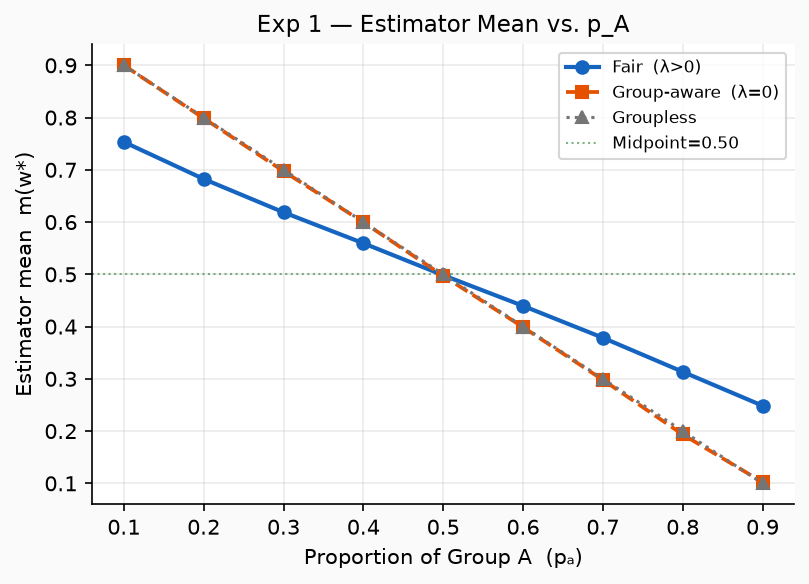
\includegraphics[width=\textwidth]{figures/exp_1_1/means.png}
        \caption{Estimator mean $\widehat{m}$ vs demographic proportion $p_A$.}
        \label{fig:exp1_1_means}
    \end{subfigure}
    \hfill
    \begin{subfigure}[b]{0.48\textwidth}
        \centering
        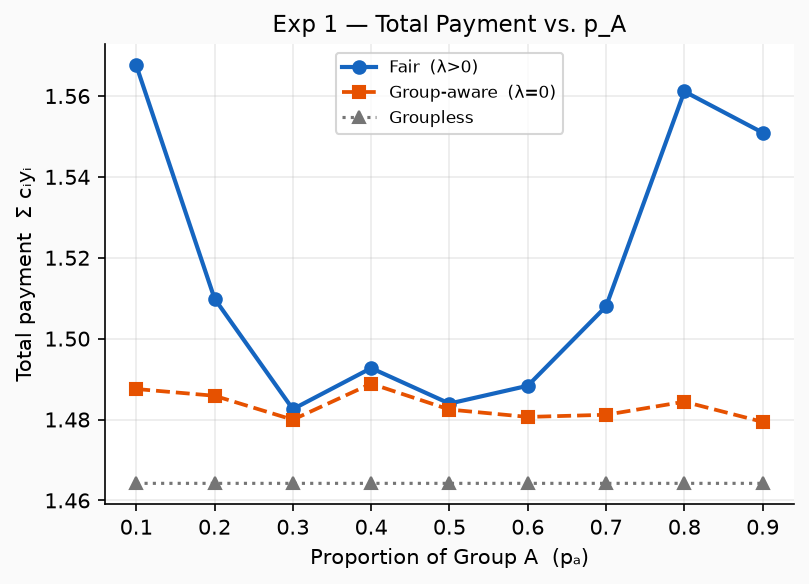
\includegraphics[width=\textwidth]{figures/exp_1_1/payments.png}
        \caption{Total payment $\sum c_i y_i$ vs demographic proportion $p_A$.}
        \label{fig:exp1_1_pay}
    \end{subfigure}
    \caption{Experiment 1: Estimator mean convergence towards midpoint and total payment behavior under varying population proportions $p_A$.}
    \label{fig:exp1_1}
\end{figure}

\subsection{Experiment 2: Varying Fairness Strength $\lambda$ (Homogeneous Costs)}

Fixing $n_A = 15, n_B = 35$ ($p_A = 0.3, p_B = 0.7 \implies \theta = 0.70$) and sweeping $\lambda \in [0, 100]$ isolates the pure effect of fairness penalty strength.

\begin{table}[htbp]
\centering
\caption{Experiment 2: Dynamics under increasing fairness strength $\lambda$ ($p_A = 0.3$, $n_A = 15, n_B = 35$, total $n = 50$).}
\label{tab:exp1_2}
\resizebox{\textwidth}{!}{%
\begin{tabular}{rrrrrrrrrrrr}
\toprule
$\lambda$ & $\widehat{m}$ & Disparity & $\MSE_{\mathrm{pop}}$ & $\MSE_A$ & $\MSE_B$ & Payment & Acquired ($N / A / B$) & $\bar{\epsilon}_A$ & $\bar{\epsilon}_B$ & $\bar{t}_A$ & $\bar{t}_B$ \\
\midrule
  0.0 & 0.6974 & 0.3947 & 0.0834 & 0.5697 & 0.1750 & 1.4800 & 25.2 / 7.9 / 17.3 & 0.1689 & 0.1667 & 0.0272 & 0.0306 \\
  0.1 & 0.6961 & 0.3921 & 0.0834 & 0.5679 & 0.1758 & 1.4799 & 25.2 / 7.9 / 17.3 & 0.1696 & 0.1664 & 0.0274 & 0.0305 \\
  0.5 & 0.6910 & 0.3821 & 0.0835 & 0.5609 & 0.1788 & 1.4798 & 25.3 / 8.0 / 17.3 & 0.1724 & 0.1652 & 0.0281 & 0.0302 \\
  1.0 & 0.6851 & 0.3702 & 0.0836 & 0.5527 & 0.1825 & 1.4797 & 25.4 / 8.1 / 17.3 & 0.1757 & 0.1638 & 0.0290 & 0.0298 \\
  2.0 & 0.6743 & 0.3486 & 0.0840 & 0.5380 & 0.1895 & 1.4799 & 25.3 / 8.2 / 17.1 & 0.1817 & 0.1612 & 0.0306 & 0.0292 \\
  5.0 & 0.6483 & 0.2965 & 0.0862 & 0.5038 & 0.2073 & 1.4808 & 25.2 / 8.2 / 17.0 & 0.1962 & 0.1549 & 0.0344 & 0.0276 \\
 10.0 & 0.6187 & 0.2374 & 0.0906 & 0.4668 & 0.2294 & 1.4826 & 25.1 / 8.4 / 16.7 & 0.2125 & 0.1478 & 0.0387 & 0.0258 \\
 50.0 & 0.5457 & 0.0914 & 0.1099 & 0.3839 & 0.2925 & 1.4983 & 24.4 / 8.9 / 15.5 & 0.2520 & 0.1297 & 0.0498 & 0.0215 \\
100.0 & 0.5258 & 0.0517 & 0.1172 & 0.3634 & 0.3117 & 1.5059 & 24.3 / 9.3 / 15.0 & 0.2624 & 0.1247 & 0.0529 & 0.0203 \\
\bottomrule
\end{tabular}%
}
\end{table}

\paragraph{Findings:}
\begin{itemize}[leftmargin=1.5em, itemsep=2pt, parsep=0pt, topsep=2pt]
    \item \textbf{Asymptotic Convergence to Midpoint:} As predicted by KKT theory, $\widehat{m} \to 0.50$ as $\lambda \to \infty$. Across the sweep, $\widehat{m}$ shifts monotonically from $0.6974$ ($\lambda = 0$) to $\mathbf{0.5258}$ ($\lambda = 100$), eliminating \textbf{87\%} of the group risk disparity ($0.3947 \to 0.0517$).
    \item \textbf{Accuracy--Fairness Risk Trade-off:} While population MSE increases from $0.0834$ to $0.1172$ due to deviation from the true population mean $\theta = 0.70$, Group A conditional MSE drops precipitously from $0.5697$ down to $0.3634$ (a $36\%$ risk reduction for the disadvantaged minority cohort), with the fairness gap collapsing by \textbf{87\%} ($0.3947 \to 0.0517$).
    \item \textbf{Acquisition and Per-Capita Payment Re-balancing:} As $\lambda$ rises from $0 \to 100$, acquired minority Group A members increase from $7.9 \to 9.3$ while majority Group B acquired drops from $17.3 \to 15.0$. Average payment to minority members $\bar{t}_A$ nearly doubles from $\$0.0272 \to \mathbf{\$0.0529}$, while majority member payment $\bar{t}_B$ declines from $\$0.0306 \to \$0.0203$. Total expenditure exhibits an initial cost dip to $\$1.4797$ at $\lambda = 1.0$ before leveling off.
\end{itemize}

\begin{figure}[H]
    \centering
    \begin{subfigure}[b]{0.48\textwidth}
        \centering
        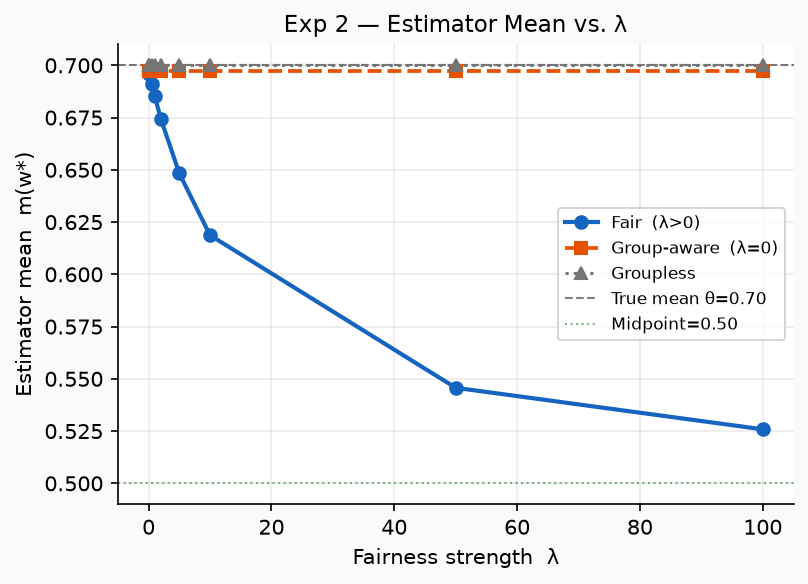
\includegraphics[width=0.85\textwidth]{figures/exp_1_2/means.png}
        \caption{Estimator mean $\widehat{m}$ vs fairness strength $\lambda$.}
        \label{fig:exp2_means}
    \end{subfigure}
    \hfill
    \begin{subfigure}[b]{0.48\textwidth}
        \centering
        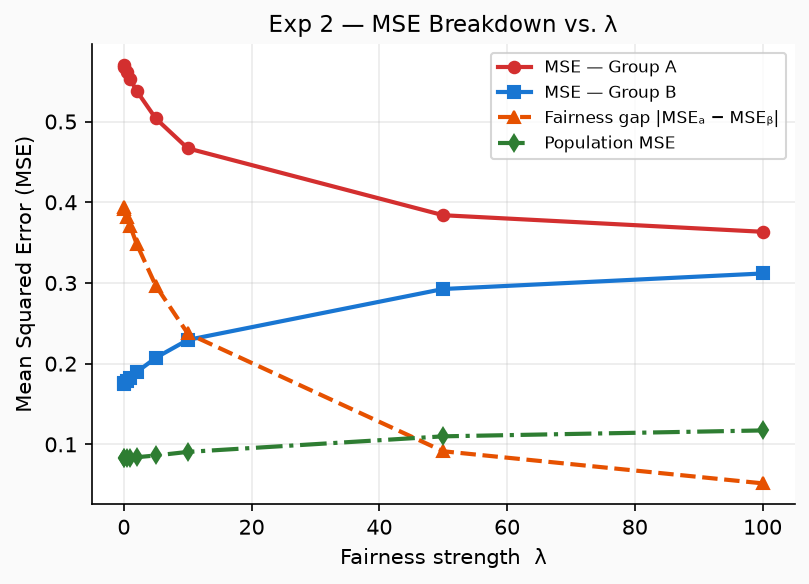
\includegraphics[width=0.85\textwidth]{figures/exp_1_2/mse.png}
        \caption{Group and population MSE vs $\lambda$.}
        \label{fig:exp2_mse}
    \end{subfigure}
    \\[0.2em]
    \begin{subfigure}[b]{0.48\textwidth}
        \centering
        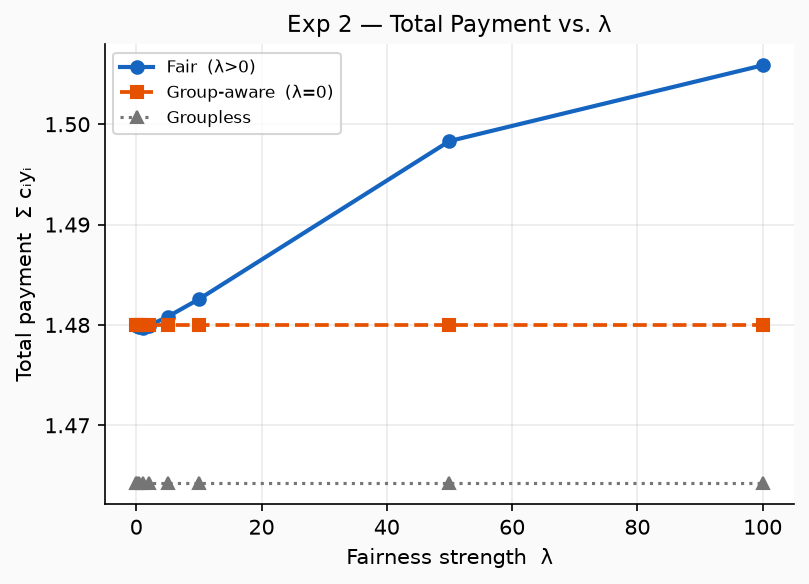
\includegraphics[width=0.85\textwidth]{figures/exp_1_2/payments.png}
        \caption{Total platform payment $\sum c_i y_i$ vs $\lambda$.}
        \label{fig:exp2_pay}
    \end{subfigure}
    \hfill
    \begin{subfigure}[b]{0.48\textwidth}
        \centering
        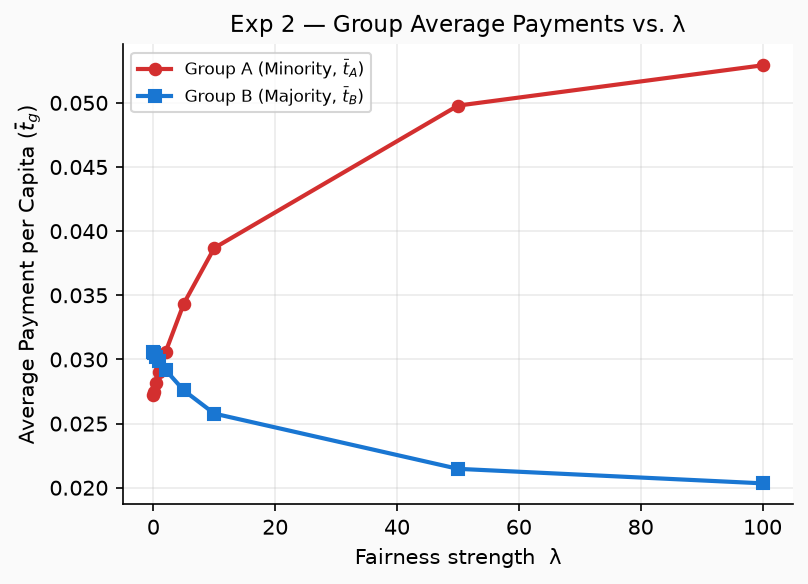
\includegraphics[width=0.85\textwidth]{figures/exp_1_2/group_payments.png}
        \caption{Average payment by group ($\bar{t}_A, \bar{t}_B$) vs $\lambda$.}
        \label{fig:exp2_group_pay}
    \end{subfigure}
    \caption{Experiment 2: Multi-metric dynamics under increasing fairness strength $\lambda$.}
    \label{fig:exp2}
\end{figure}

\FloatBarrier
\clearpage

\subsection{Experiment 3: Inter-Group Privacy Cost Disparity}
\label{sec:exp2-1}
We introduce systematic cost asymmetry: Group A represents individuals with cheap privacy ($\bar{c}_A = 0.5$), while Group B represents individuals with elevated privacy costs ($\bar{c}_B \geq 0.5$).  \emph{Note: The Groupless estimator is omitted because group-blind acquisition is theoretically invalid when costs depend on group identity ($c_i \sim F_{g(i)}$). The group model enables us to handle such cases where certain groups have higher cost to privacy.}


\subsubsection{Varying Cost Disparity Ratio (Equal Proportions $p_A = p_B = 0.5$)}

We hold $n_A = n_B = 25$ and vary the cost ratio $c_B/c_A \in [1.0, 20.0]$ ($\bar{c}_B \in [0.5, 10.0]$) at fairness strength $\lambda = 10.0$.

\begin{table}[htbp]
\centering
\caption{Experiment 3.1: Cost ratio sweep with equal demographic sizes ($n_A = 25, n_B = 25$, total $n = 50$, $\lambda = 10.0$).}
\label{tab:exp2_1_1}
\resizebox{\textwidth}{!}{%
\begin{tabular}{lrrrrrrrrr}
\toprule
Estimator & $\widehat{m}$ & Disparity & $\MSE_{\mathrm{pop}}$ & Payment & Acquired ($N / A / B$) & $\bar{\epsilon}_A$ & $\bar{\epsilon}_B$ & $\bar{t}_A$ & $\bar{t}_B$ \\
\midrule
\multicolumn{10}{l}{\textbf{Cost Ratio $c_B/c_A = 1.0$} \quad ($\bar{c}_A = 0.5, \bar{c}_B = 0.50$, \ Pool: $25$ A, $25$ B)} \\
\midrule
Fair         & 0.4998 & 0.0086 & 0.0823 & 1.4673 & 26.5 / 12.5 / 14.0 & 0.1694 & 0.1694 & 0.0279 & 0.0308 \\
Group-Aware  & 0.4996 & 0.0145 & 0.0823 & 1.4659 & 26.4 / 12.5 / 13.9 & 0.1695 & 0.1694 & 0.0279 & 0.0307 \\
\midrule
\multicolumn{10}{l}{\textbf{Cost Ratio $c_B/c_A = 5.0$} \quad ($\bar{c}_A = 0.5, \bar{c}_B = 2.50$, \ Pool: $25$ A, $25$ B)} \\
\midrule
Fair         & 0.4496 & 0.1008 & 0.1233 & 1.9914 & 20.1 / 14.1 / 6.0 & 0.1615 & 0.1330 & 0.0300 & 0.0496 \\
Group-Aware  & 0.4169 & 0.1662 & 0.1252 & 1.9086 & 19.5 / 14.1 / 5.4 & 0.1736 & 0.1257 & 0.0331 & 0.0432 \\
\midrule
\multicolumn{10}{l}{\textbf{Cost Ratio $c_B/c_A = 10.0$} \quad ($\bar{c}_A = 0.5, \bar{c}_B = 5.00$, \ Pool: $25$ A, $25$ B)} \\
\midrule
Fair         & 0.4161 & 0.1678 & 0.1517 & 2.0223 & 17.6 / 14.2 / 3.4 & 0.1707 & 0.1223 & 0.0334 & 0.0475 \\
Group-Aware  & 0.3700 & 0.2600 & 0.1519 & 1.9305 & 17.8 / 14.6 / 3.2 & 0.1865 & 0.1108 & 0.0375 & 0.0397 \\
\midrule
\multicolumn{10}{l}{\textbf{Cost Ratio $c_B/c_A = 20.0$} \quad ($\bar{c}_A = 0.5, \bar{c}_B = 10.00$, \ Pool: $25$ A, $25$ B)} \\
\midrule
Fair         & 0.3884 & 0.2233 & 0.1710 & 2.3355 & 17.9 / 15.2 / 2.7 & 0.1662 & 0.1068 & 0.0348 & 0.0587 \\
Group-Aware  & 0.3289 & 0.3422 & 0.1734 & 2.1193 & 18.0 / 15.7 / 2.3 & 0.1889 & 0.0941 & 0.0407 & 0.0441 \\
\bottomrule
\end{tabular}%
}
\end{table}

\paragraph{Findings:}
\begin{itemize}[leftmargin=1.5em]
    \item \textbf{Cost-Driven Disparity Emergence:} Even when groups have identical sizes ($p_A = p_B = 0.5$), cost asymmetry drives the unconstrained estimator ($\lambda = 0$) to aggressively substitute cheap Group A data for expensive Group B data. At a steep $20\times$ ratio ($\bar{c}_B = 10.0$), $\widehat{m}$ plunges to $0.3289$, resulting in a disparity of $0.3422$.
    \item \textbf{Counter-Acting Economic Pressure ($\lambda = 10.0$):} The fair estimator actively resists this economic distortion, preserving allocations to expensive Group B ($\bar{\epsilon}_B = 0.1068$ with 2.7 active participants) and maintaining a significantly more balanced mean ($\widehat{m} = \mathbf{0.3884}$ vs $0.3289$), slashing the disparity from $0.3422 \to 0.2233$ (a 35\% reduction).
\end{itemize}

\begin{figure}[htbp]
    \centering
    \begin{subfigure}[b]{0.48\textwidth}
        \centering
        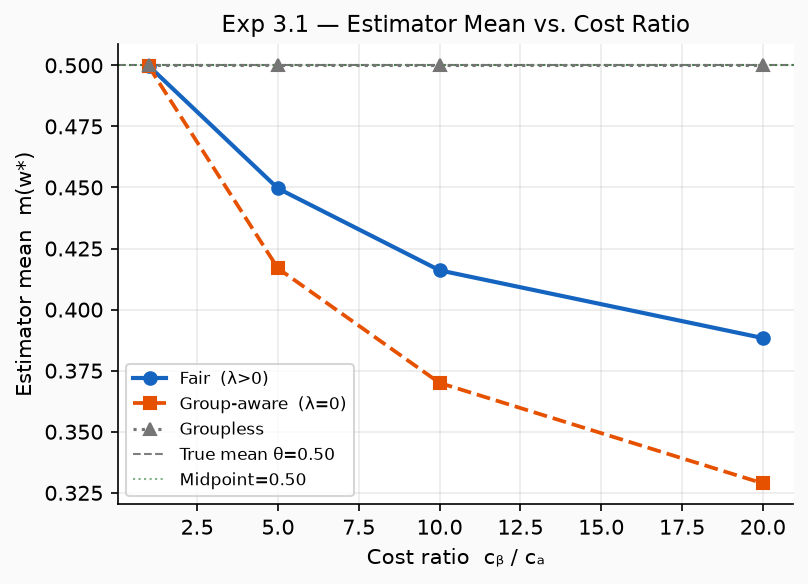
\includegraphics[width=\textwidth]{figures/exp_2_1_1/means.png}
        \caption{Estimator mean $\widehat{m}$ vs cost ratio $c_B/c_A$.}
        \label{fig:exp2_1_1_means}
    \end{subfigure}
    \hfill
    \begin{subfigure}[b]{0.48\textwidth}
        \centering
        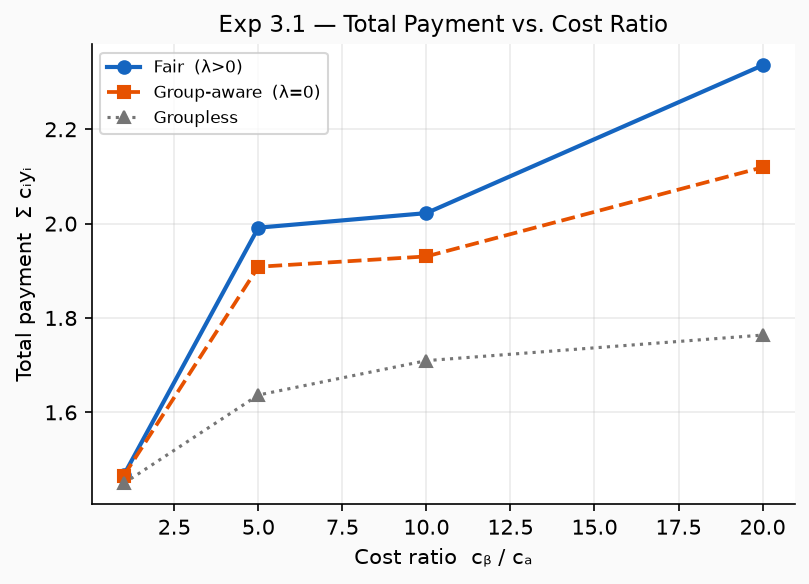
\includegraphics[width=\textwidth]{figures/exp_2_1_1/payments.png}
        \caption{Total payments vs cost ratio $c_B/c_A$.}
        \label{fig:exp2_1_1_pay}
    \end{subfigure}
    \caption{Experiment 3.1: Distortion of estimator mean driven purely by cost disparity and fair estimator compensation behavior.}
    \label{fig:exp2_1_1}
\end{figure}

\subsubsection{Varying Demographic Proportions with Fixed Cost Disparity ($c_B = 3 c_A$)}

We fix $\bar{c}_A = 0.5, \bar{c}_B = 1.5$ ($3\times$ ratio) at fairness strength $\lambda = 10.0$ and sweep $p_A \in [0.1, 0.9]$.

\begin{table}[htbp]
\centering
\caption{Experiment 3.2: Demographic sweep under heterogeneous costs ($\bar{c}_A = 0.5, \bar{c}_B = 1.5$, total $n = 50$, $\lambda = 10.0$).}
\label{tab:exp2_1_2}
\resizebox{\textwidth}{!}{%
\begin{tabular}{lrrrrrrrrr}
\toprule
Estimator & $\widehat{m}$ & Disparity & $\MSE_{\mathrm{pop}}$ & Payment & Acquired ($N / A / B$) & $\bar{\epsilon}_A$ & $\bar{\epsilon}_B$ & $\bar{t}_A$ & $\bar{t}_B$ \\
\midrule
\multicolumn{10}{l}{\textbf{Minority Cheap Group A (Majority Expensive B)} \quad ($p_A = 0.1$, \ Pool: $n_A = 5, n_B = 45$, \ Target $\theta = 0.90$)} \\
\midrule
Fair         & 0.7272 & 0.4544 & 0.1526 & 2.0683 & 17.2 / 4.3 / 12.9 & 0.3889 & 0.1157 & 0.1220 & 0.0324 \\
Group-Aware  & 0.8601 & 0.7202 & 0.1269 & 2.1165 & 17.3 / 3.3 / 14.0 & 0.1972 & 0.1362 & 0.0475 & 0.0418 \\
\midrule
\multicolumn{10}{l}{\textbf{Equal Representation} \quad ($p_A = 0.5$, \ Pool: $n_A = 25, n_B = 25$, \ Target $\theta = 0.50$)} \\
\midrule
Fair         & 0.4688 & 0.0624 & 0.1075 & 1.8289 & 20.9 / 13.3 / 7.6 & 0.1623 & 0.1438 & 0.0290 & 0.0441 \\
Group-Aware  & 0.4485 & 0.1031 & 0.1081 & 1.7996 & 21.0 / 13.4 / 7.6 & 0.1694 & 0.1387 & 0.0308 & 0.0412 \\
\midrule
\multicolumn{10}{l}{\textbf{Majority Cheap Group A (Minority Expensive B)} \quad ($p_A = 0.9$, \ Pool: $n_A = 45, n_B = 5$, \ Target $\theta = 0.10$)} \\
\midrule
Fair         & 0.1972 & 0.6055 & 0.1097 & 2.1050 & 25.9 / 23.1 / 2.8 & 0.1263 & 0.2806 & 0.0231 & 0.2133 \\
Group-Aware  & 0.0435 & 0.9130 & 0.0904 & 1.5896 & 25.0 / 23.9 / 1.1 & 0.1717 & 0.0704 & 0.0320 & 0.0297 \\
\bottomrule
\end{tabular}%
}
\end{table}

\paragraph{Findings:}
\begin{itemize}[leftmargin=1.5em]
    \item \textbf{Validation of the ``Cheaper Fairness'' Phenomenon:} When the expensive group B is also the demographic majority ($p_A = 0.1$, so $90\%$ of the population belongs to B), fair estimation yields a win-win situation: it reduces group MSE disparity by \textbf{37\%} (from $0.7202$ down to $0.4544$) while simultaneously \textbf{reducing procurement payment} from $\$2.1165$ down to $\mathbf{\$2.0683}$. Because majority group B individuals carry high virtual costs ($\psi_B = 2c_B$), de-allocating privacy from 14.0 majority participants down to 12.9 saves more money than the compensation needed to boost minority Group A allocations ($\bar{\epsilon}_A$ increases from $0.1972 \to 0.3889$, with $\bar{t}_A$ rising from $\$0.0475 \to \$0.1220$).
    \item \textbf{Asymmetric Cost Dynamics at $p_A = 0.9$:} Conversely, when the expensive group is a tiny minority ($p_A = 0.9, n_B = 5$), achieving fairness requires aggressively purchasing privacy from expensive Group B participants ($\bar{\epsilon}_B$ increases fourfold from $0.0704 \to 0.2806$, and active participants increase from $1.1 \to 2.8$). This causes average compensation to minority B members to surge more than sevenfold from $\$0.0297 \to \mathbf{\$0.2133}$, driving total platform payment from $\$1.5896 \to \$2.1050$.
\end{itemize}

\begin{figure}[htbp]
    \centering
    \begin{subfigure}[b]{0.48\textwidth}
        \centering
        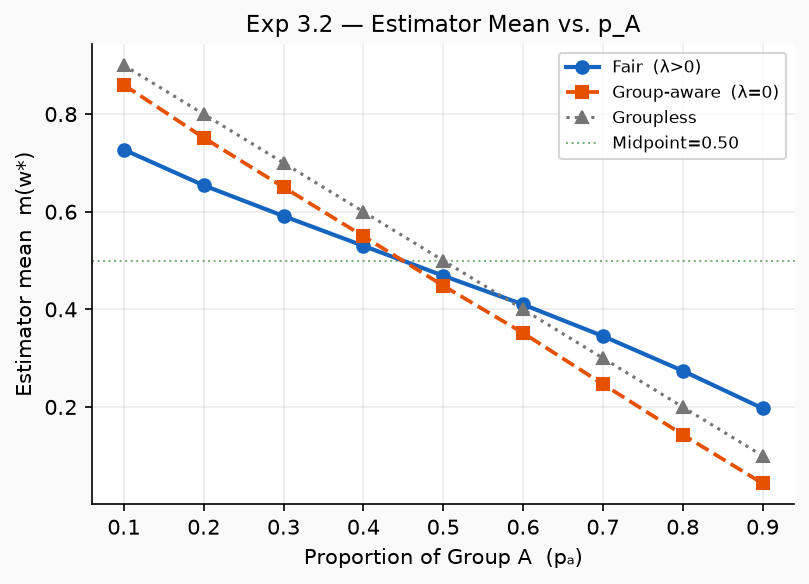
\includegraphics[width=\textwidth]{figures/exp_2_1_2/means.png}
        \caption{Estimator mean $\widehat{m}$ vs $p_A$ under $c_B = 3c_A$.}
        \label{fig:exp2_1_2_means}
    \end{subfigure}
    \hfill
    \begin{subfigure}[b]{0.48\textwidth}
        \centering
        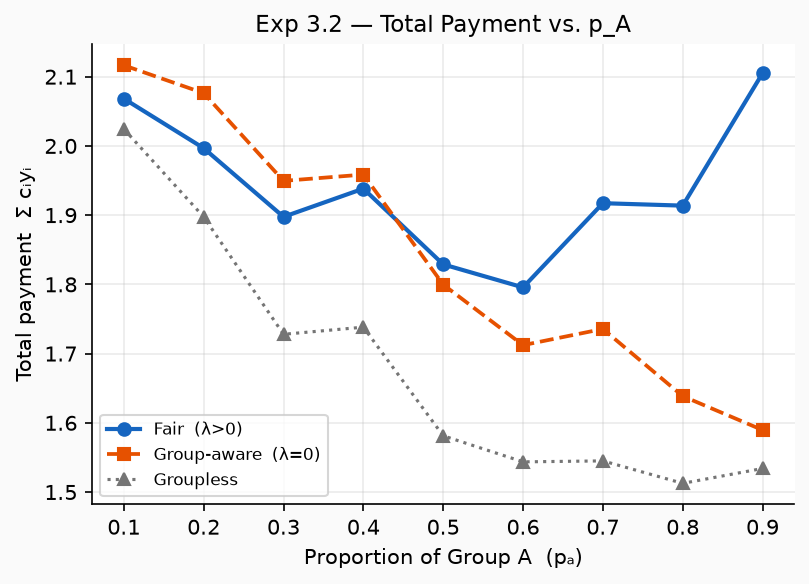
\includegraphics[width=\textwidth]{figures/exp_2_1_2/payments.png}
        \caption{Total payment vs $p_A$ under $c_B = 3c_A$ (showing cost reduction at $p_A = 0.1$).}
        \label{fig:exp2_1_2_pay}
    \end{subfigure}
    \caption{Experiment 3.2: Interaction of demographic proportion sweep with asymmetric privacy costs ($\lambda = 10.0$).}
    \label{fig:exp2_1_2}
\end{figure}

\subsection{Experiment 4: Comparison of Privacy Cost Distributions}

We examine how the distributional shape of privacy costs impacts optimal procurement when first and second moments are held fixed ($\bar{c}_A = 0.5, \bar{c}_B = 1.0, \Var(c) = \bar{c}^2/3, \lambda = 10.0, n_A = n_B = 25$).

\begin{table}[htbp]
\centering
\caption{Experiment 4: Distribution comparison with matched first and second moments ($n_A = 25, n_B = 25$, total $n = 50$, $\lambda = 10.0$).}
\label{tab:exp2_2}
\resizebox{\textwidth}{!}{%
\begin{tabular}{lrrrrrrrrr}
\toprule
Estimator & $\widehat{m}$ & $\MSE_{\mathrm{pop}}$ & Disparity & Payment & Acquired ($N / A / B$) & $\bar{\epsilon}_A$ & $\bar{\epsilon}_B$ & $\bar{t}_A$ & $\bar{t}_B$ \\
\midrule
\multicolumn{10}{l}{\textbf{Uniform Distribution} \quad ($\bar{c}_A = 0.5, \bar{c}_B = 1.0, \Var(c) = \bar{c}^2/3$)} \\
\midrule
Fair         & 0.4819 & 0.0967 & 0.0363 & 1.6945 & 22.5 / 13.1 / 9.4 & 0.1639 & 0.1528 & 0.0285 & 0.0393 \\
Group-Aware  & 0.4697 & 0.0970 & 0.0606 & 1.6816 & 22.6 / 13.3 / 9.3 & 0.1681 & 0.1495 & 0.0295 & 0.0377 \\
\midrule
\multicolumn{10}{l}{\textbf{Log-Normal Distribution} \quad ($\bar{c}_A = 0.5, \bar{c}_B = 1.0, \Var(c) = \bar{c}^2/3$)} \\
\midrule
Fair         & 0.4805 & 0.0855 & 0.0391 & 2.8669 & 29.0 / 16.5 / 12.5 & 0.1464 & 0.1354 & 0.0423 & 0.0724 \\
Group-Aware  & 0.4669 & 0.0859 & 0.0663 & 2.8477 & 29.5 / 16.7 / 12.8 & 0.1509 & 0.1322 & 0.0437 & 0.0702 \\
\midrule
\multicolumn{10}{l}{\textbf{Truncated Normal Distribution} \quad ($\bar{c}_A = 0.5, \bar{c}_B = 1.0, \Var(c) = \bar{c}^2/3$)} \\
\midrule
Fair         & 0.4816 & 0.0927 & 0.0368 & 2.0352 & 25.3 / 14.4 / 10.9 & 0.1570 & 0.1461 & 0.0335 & 0.0479 \\
Group-Aware  & 0.4691 & 0.0931 & 0.0619 & 2.0197 & 25.0 / 14.4 / 10.6 & 0.1612 & 0.1428 & 0.0347 & 0.0461 \\
\bottomrule
\end{tabular}%
}
\end{table}

\paragraph{Findings:}
\begin{itemize}[leftmargin=1.5em]
    \item \textbf{Heavy-Tail Payment Escalation:} Despite identical mean and variance, the Log-Normal cost distribution demands dramatically higher expected total payments ($2.8669$) compared to Uniform ($1.6945$) and Truncated Normal ($2.0352$). The unbounded right tail forces severe informational rents via virtual costs $\psi_i$.
    \item \textbf{Robustness of the Estimator Mean:} Remarkably, the optimal fair mean $\widehat{m}$ remains virtually identical across all three distribution geometries ($0.4805 \le \widehat{m} \le 0.4819$), and the fairness disparity is clamped to $\approx 0.036$--$0.039$ across all three. This demonstrates empirically that optimal fair aggregation weights are dictated by first and second moments rather than higher-order tail behavior.
\end{itemize}

\begin{figure}[htbp]
    \centering
    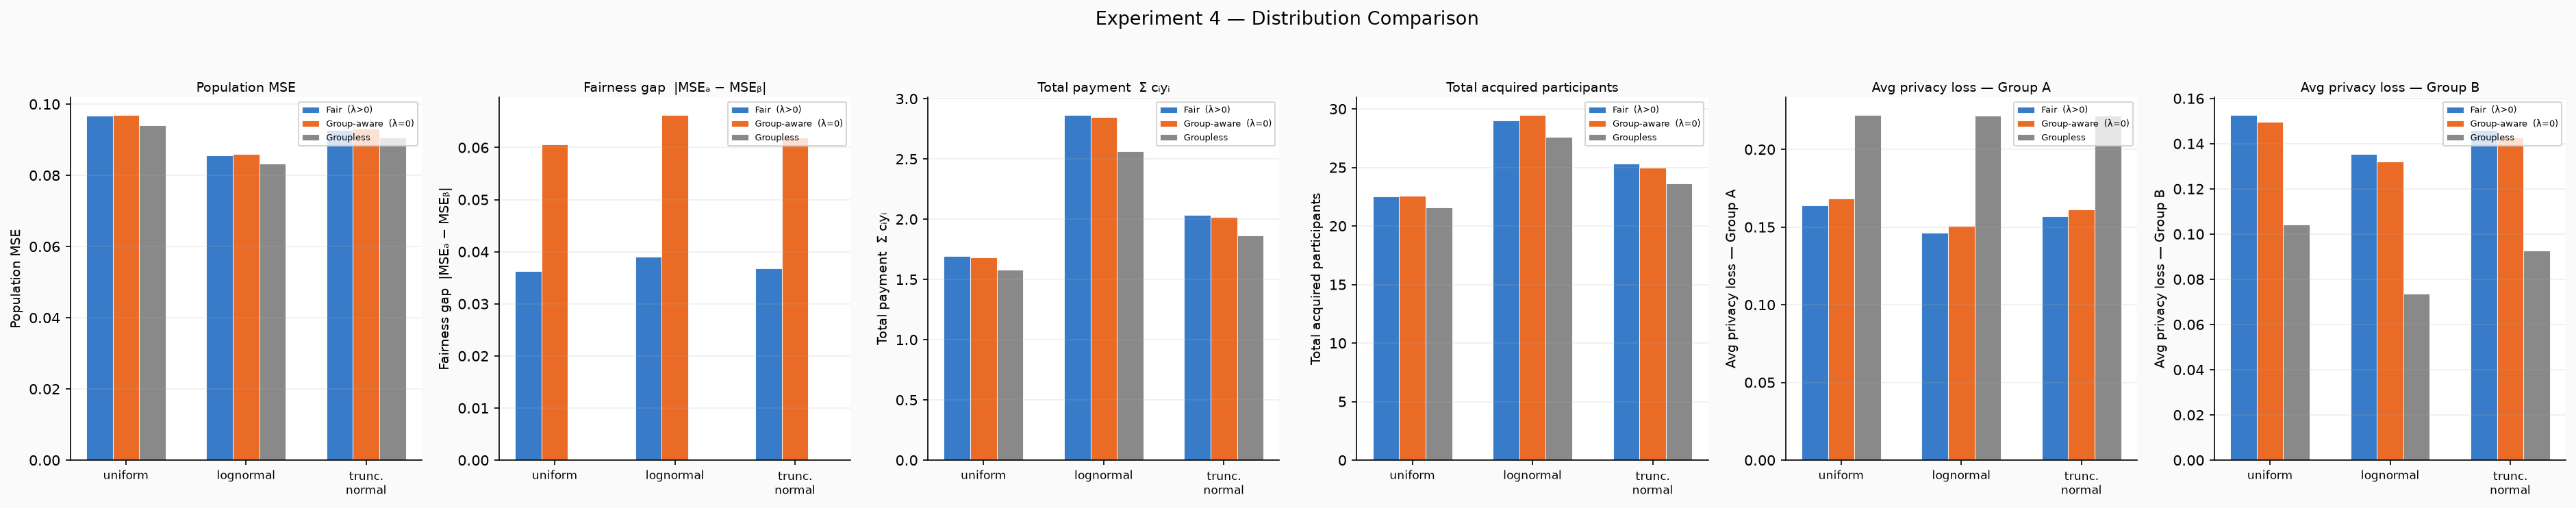
\includegraphics[width=\textwidth]{figures/exp_2_2/comparison.png}
    \caption{Experiment 4: Side-by-side comparison across Uniform, Log-Normal, and Truncated Normal privacy cost distributions across population MSE, fairness gap, total payments, and group privacy loss allocations.}
    \label{fig:exp2_2}
\end{figure}

%=============================================================================
\section{The ``Cheaper Fairness'' Phenomenon: Mechanism and Intuition}
%=============================================================================

One of the most curious findings in this study is that incorporating a fairness objective does \textbf{not} universally increase the platform's procurement costs. In fact, under moderate penalties or when the demographic majority carries higher privacy costs (as observed prominently in Experiment 3.2 and for moderate $\lambda$ in Experiment 2), we observe:
\begin{equation}
    \text{Payment}(\lambda > 0) < \text{Payment}(\lambda = 0).
\end{equation}

\subsection{Analytical Decomposition}

Total expected procurement payments are given by $P = S \sum_i \psi_i w_i = \sum_i \psi_i y_i$. Differentiating total payment with respect to fairness strength $\lambda$:
\begin{equation}
    \frac{\partial P}{\partial \lambda} = \sum_{i \in \mathcal{A}} \psi_i \frac{\partial y_i}{\partial \lambda} + \sum_{j \in \mathcal{B}} \psi_j \frac{\partial y_j}{\partial \lambda}.
\end{equation}
Suppose Group B is the demographic majority ($n_B > n_A$) and has a higher group mean $\mu_B > \mu_A$. Without fairness ($\lambda = 0$), the optimal weights align with population proportions, placing heavy aggregate weight on Group B ($m(w^*) \approx \theta > (\mu_A+\mu_B)/2$).

To satisfy the fairness condition, $m(w^*)$ must decrease toward the midpoint. This requires:
\begin{equation}
    \sum_{i \in \mathcal{A}} \frac{\partial y_i}{\partial \lambda} > 0, \qquad \sum_{j \in \mathcal{B}} \frac{\partial y_j}{\partial \lambda} < 0.
\end{equation}
Because the marginal reduction in MSE bias penalty is quadratic, the mechanism disproportionately contracts the allocations $y_j$ of the numerous majority members in Group B:
\begin{equation}
    n_B \left| \Delta \bar{y}_B \right| > n_A \left| \Delta \bar{y}_A \right|.
\end{equation}
When the savings from shedding majority privacy loss exceed the extra payment needed to incentivize minority participation, net payment strictly falls:
\begin{equation}
    \Delta P \approx n_A \bar{\psi}_A \Delta \bar{y}_A - n_B \bar{\psi}_B |\Delta \bar{y}_B| < 0.
\end{equation}

\subsection{Characterization of the Regimes}

Fairness reduces procurement costs under two distinct structural regimes:
\begin{enumerate}
    \item \textbf{Demographic Asymmetry (Exp 1, Exp 2):} When the majority group is large ($p_B \gg p_A$), equalizing representation requires throttling majority privacy expenditure, saving significant money on the bulk cohort.
    \item \textbf{Cost Disparity with Majority Concentration (Exp 3.2):} When the demographic majority also possesses higher privacy costs ($\bar{c}_B > \bar{c}_A$), the cost-saving effect of de-allocating privacy from the majority is magnified by their higher virtual cost rate $\psi_B > \psi_A$.
\end{enumerate}

%=============================================================================
\section{Discussion, Limitations, and Future Work}
%=============================================================================

\subsection{Algorithmic Considerations}

While our SLSQP optimizer with multi-start initialization provided stable and robust solutions across all $n \leq 100$ settings in seconds, the theoretical algorithm derives an exact $O(n \log n)$ threshold-sweep algorithm for the standard mechanism. As detailed in our derivations:
\begin{itemize}[leftmargin=1.5em]
    \item The two-threshold consistency path $\tau_B = g(\tau_A)$ is piecewise linear with at most $n+1$ active segments.
    \item On each segment, the outer stationarity condition collapses to a quartic polynomial in $\tau_A$:
    \begin{equation}
        4(n+1)(h_0 + h_1\tau_A)^4 - K^3(u_0 + u_1\tau_A) = 0.
    \end{equation}
    Future work should implement an exact algebraic quartic root solver that verifies the active-set boundary conditions to scale the mechanism to $n \geq 10^5$ participants.
\end{itemize}

\subsection{Theoretical Limitations}

\begin{enumerate}
    \item \textbf{Identical Within-Group Variance:} Our current formulation assumes $\Var(X_i) = \sigma^2$ across both groups. If groups exhibit unequal variances ($\sigma_A^2 \neq \sigma_B^2$), subtracting conditional MSEs no longer eliminates the variance term, introducing cross-terms $w_i^2$ into the fairness penalty and destroying the affine consistency path.
    \item \textbf{Two-Group Restriction:} Extending demographic fairness beyond two groups ($K > 2$) introduces pairwise disparity penalties $\sum_{j < k} D_{jk}(w)^2$, which transforms the 1D threshold path into a coupled $(K-1)$-dimensional manifold.
\end{enumerate}

%=============================================================================
\section{Conclusion}
%=============================================================================

This report presented an end-to-end mechanism-design and empirical study of fairness-augmented differentially private data acquisition. By incorporating group-conditional MSE penalties, the platform successfully balances empirical fidelity against demographic fairness. Our experimental results across five distinct test configurations confirm theoretical predictions: the estimator mean interpolates smoothly from the population mean to the group midpoint. Crucially, we demonstrated that achieving fairness is not inherently economically expensive: under widespread demographic or cost asymmetries, fair allocation may actively reduce the buyer's procurement bill by pruning redundant majority privacy loss.

%=============================================================================
% References
%=============================================================================
\begin{thebibliography}{99}

\bibitem{fallah2023optimal}
A.~Fallah, A.~Makhdoumi, A.~Malekian, and A.~Ozdaglar.
\newblock Optimal and differentially private data acquisition: Central and local mechanisms.
\newblock {\em Operations Research}, 71(5):1748--1768, 2023.

\bibitem{dwork2006calibrating}
C.~Dwork, F.~McSherry, K.~Nissim, and A.~Smith.
\newblock Calibrating noise to sensitivity in private data analysis.
\newblock In {\em Theory of Cryptography Conference (TCC)}, volume 3876 of {\em Lecture Notes in Computer Science}, pages 265--284. Springer, 2006.

\bibitem{dwork2014algorithmic}
C.~Dwork and A.~Roth.
\newblock The algorithmic foundations of differential privacy.
\newblock {\em Foundations and Trends in Theoretical Computer Science}, 9(3--4):211--407, 2014.

\bibitem{myerson1981optimal}
R.~B. Myerson.
\newblock Optimal auction design.
\newblock {\em Mathematics of Operations Research}, 6(1):58--73, 1981.

\end{thebibliography}

\end{document}
